\section{General Architecture \& Code Generation}
\label{sec:CG}

Fundamentally, \IOTDSL describes a real-time reactive system: information is regularly reported to the middleware where it is processed in order to react on the environment. However, in the context of \IOT systems, the environment cannot be controlled, but it is perceived through the many deployed devices, that allow at the same time to react on it. The key task is then to process events quickly enough to ensure appropriate reactions, although it it not critical to react in a precise timeframe. In this section, we first describe the general architecture of our tool as well as the technical choices for processing events in an \IOT system, then provide a compilation schema to translate \IOTDSL business rules into Tesla rules, the entry language of TRex \cite{cugola-12}, the \CEP engine we have chosen in our architecture.

\subsection{General Architecture}
\label{sec:CG-Architecture}

As many \IOT solutions, \IOTDSL massively relies on event processing. In order to transform abstract event definitions into runnable code, we rely on a middleware on which the event processing will run and that will be responsible for the evaluation of the rules. Figure~\ref{fig:gen-archi} depicts the general architecture of the \IOTDSL framework.

\begin{figure}%
	\centering  
	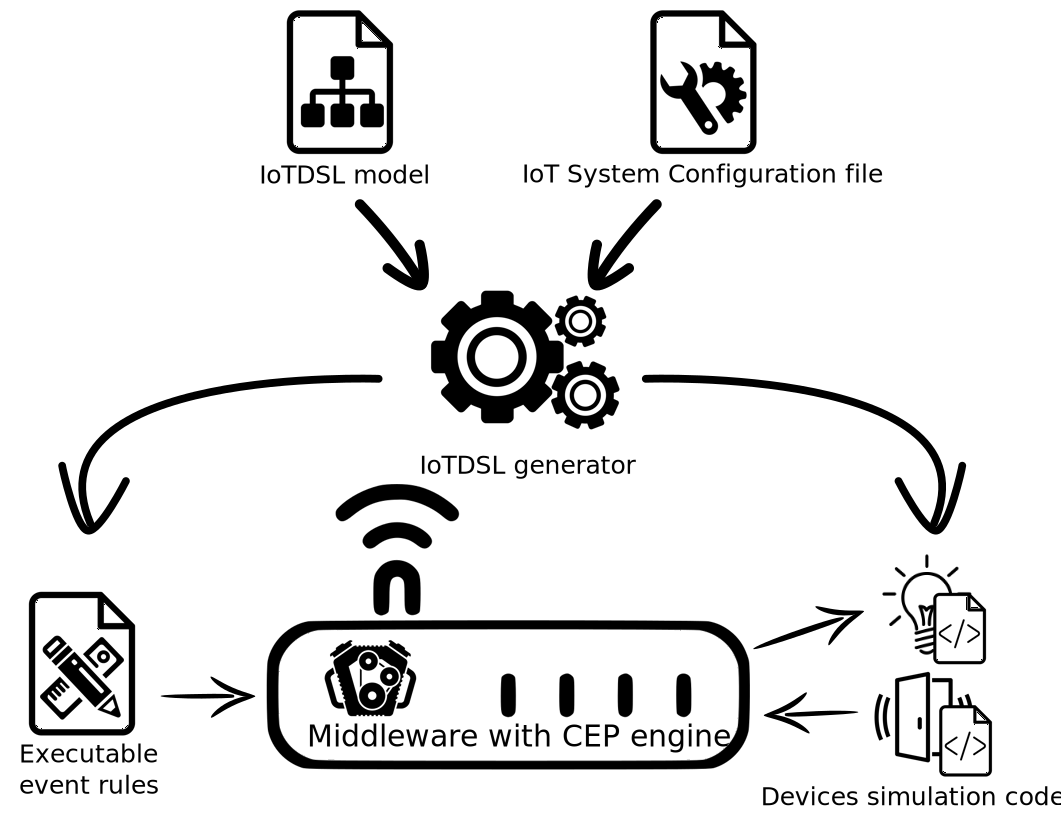
\includegraphics[width=.9\linewidth]{gen-archi.png}%
	\caption{General architecture of \IOTDSL framework}%
	\label{fig:gen-archi}%
\end{figure}


\subsection{TRex as \CEP engine}
\label{sec:CG-TRex}

To permit efficient event processing from distributed connected things, we rely on TRex, a powerful and highly optimised \CEP engine developed by Cugola and Margara~\cite{cugola-12}. TRex relies on Tesla \cite{Cugola-Margara:2010}, an entry language that is expressive enough to address most of the necessary patterns for capturing complex events definitions. As a consequence, the expression language used for triggers in our business rules is directly inspired from Tesla. This allows us to offer end-users the expressibility they need, while at the same time simplifying the translation of \IOTDSL rules into Tesla rules. TRex offers a queueing mechanism to overcome bursts of incoming events: when deploying the \IOT system on site, it becomes possible to customise the queue size, thus balancing between event loss and treatment latency. 

TRex is conveniently organised as a Client/Server architecture in a \textit{<<publish / subscribe>>} way: on the server side, event notifications are received at runtime, and processed according to a set of rules defined in the Tesla language, resulting in the production of a hierarchy of complex events that could be reused internally, whereas clients subscribe to the server with the event notifications they are interested in. Note that the server is interactive so that clients can (un-)subscribe while the engine is running and rules may be added or deleted at runtime without affecting the overall infrastructure. 

From the perspective of \IOTDSL, TRex offers several benefits as a \CEP engine middleware: TRex is powerful enough to handle typical \IOT scenarios like the one described in Section \ref{sec:Motivation}, thanks to the expressive power of Tesla. It adopts a decentralised architecture that directly reflects our design choices, and supports distributed processing of events to reduce the cost of communication and to optimise resource usage. It is developed in C, so it is even suitable for \textit{small form factor} middlewares. Finally, on top of a C \textsc{API}, Java libraries have been developed on which we rely to generate devices' simulation code.

\subsection{Compiling \IOTDSL Rules}
\label{sec:CG-Compilation}

